%% neanderthal_2016.tex
%% Author: Leighton Pritchard
%% Copyright: James Hutton Institute
%% Example slides: Comparative Genomics In The News 2016

%
\begin{frame}
  \frametitle{Comparative genomics in the news
                   \footnote{\tiny{\href{http://www.bbc.co.uk/news/science-environment-35806992}{BBC News 15/3/2016
}}}
                   \footnote{\tiny{\href{http://dx.doi.org/10.1038/nature17405
}{Meyer \textit{et al}. (2016) \textit{Nature} doi:10.1038/nature17405
}}}
}
    \begin{columns}[c] 
      \column{.6\textwidth} 
        \begin{itemize}
          \item \textcolor{RawSienna}{Oldest DNA ever recovered from a human (430kya) - 0.1\% of genome}
          \item \textcolor{hutton_blue}{28 individuals, Sima de los Huesos, N. Spain}
          \item \textcolor{hutton_purple}{mitoDNA more similar to Siberian Denisovans than to modern humans}
          \item \textcolor{hutton_green}{Modern humans derived from wave out of Africa 250kya, with mitochondrial turnover?}
        \end{itemize}
      \column{.4\textwidth}
        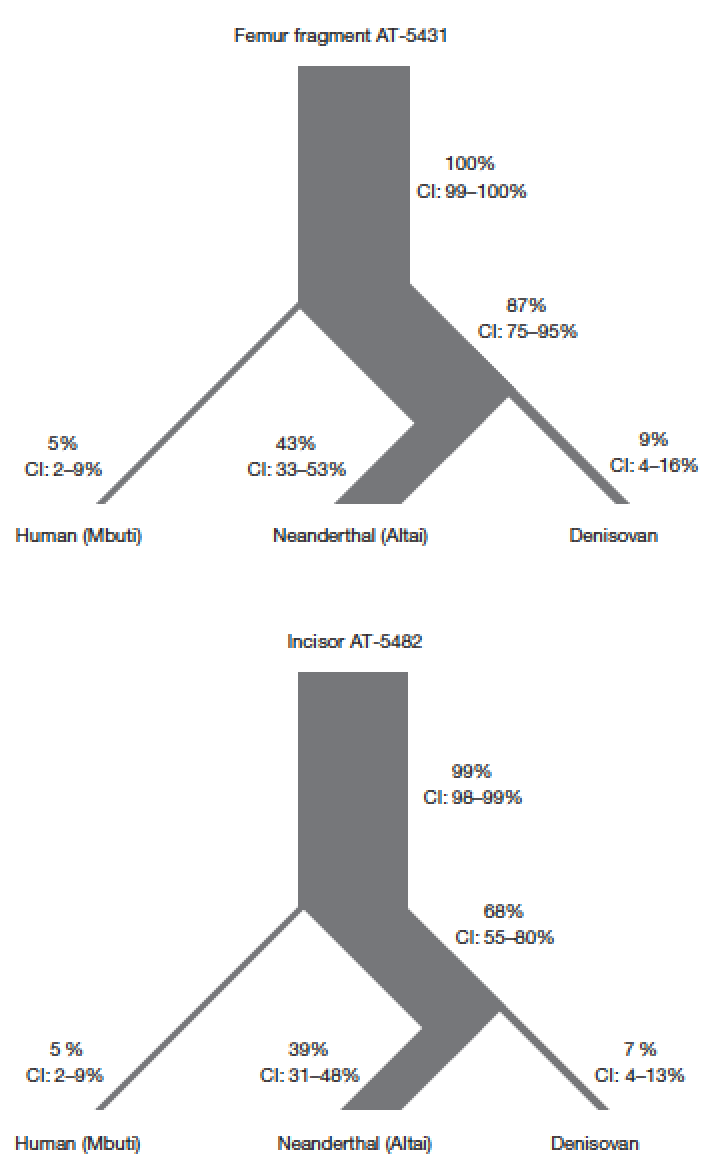
\includegraphics[width=\textwidth]{images/sima_shared} \\
        %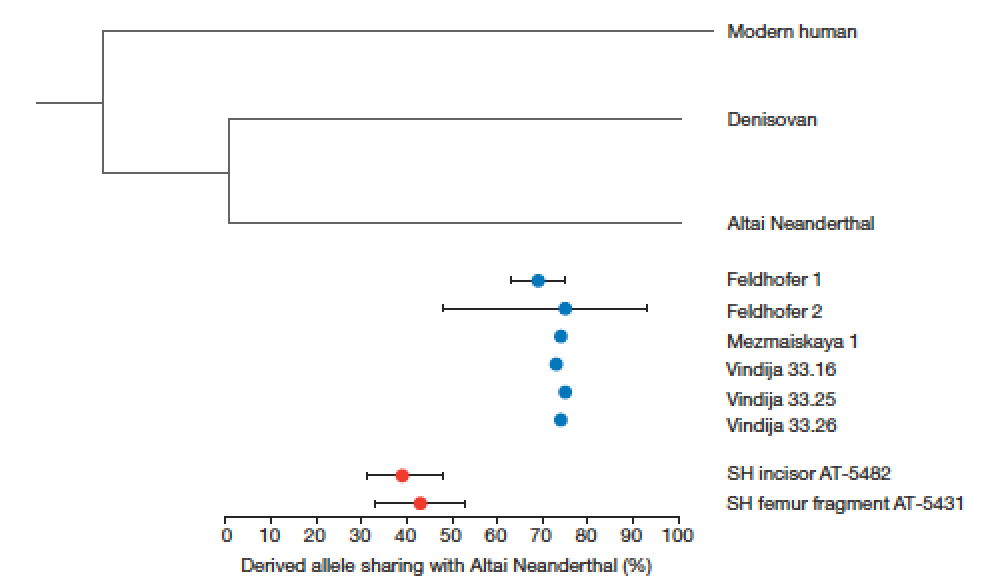
\includegraphics[width=\textwidth]{images/sima_tree}
    \end{columns}  
\end{frame}